\documentclass[]{article}

\title{Memoria de la práctica 1 \\
	\Large Sistemas operativos 2018-2019}

\author{Alejandro Pascual y V\'ictor Yrazusta}
\usepackage{amssymb}
\usepackage{graphicx}
\usepackage[spanish, es-tabla]{babel}
\usepackage[legalpaper, margin=1in]{geometry}

\begin{document}

\maketitle

\section*{Respuestas a las preguntas cortas}
\subsection*{Ejercicio 3}
\subsubsection*{a)}
No se puede saber cual se ejecuta antes,
ya que el padre no espera a la ejecución del hijo.

\subsubsection*{b)}
Lo hemos hecho usando las funciones \textit{getpid()} y \textit{getppid()}.

\subsubsection*{c)}
\begin{center}
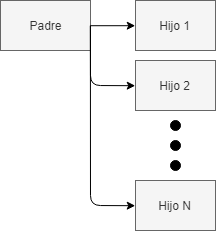
\includegraphics[scale=0.75]{3c.png}
\end{center}
El padre va creando procesos hijos y no espera a que estos terminen su ejecución para terminar él la suya, de manera que deja hijos huérfanos. 

\subsection*{Ejercicio 4}
\subsubsection*{a)}
El padre puede dejar 2 hijos huérfanos al solo tener un \textit{wait()} e iniciar 3 procesos hijo.

\subsubsection*{b)}
Los cambios se limitan a introducir un \textit{wait()} dentro del bucle en el que el padre va creando procesos.

\subsection*{Ejercicio 5}
\subsubsection*{a)}
El padre no imprime el valor al que el hijo ha inicializado la variable. Suponemos que esto se debe a que, cuando se ejecuta \textit{fork()}, se trata de la misma forma a la memoria dinámica y a la estática, generando una nueva copia para el proceso hijo.

\subsubsection*{b)}
La respuesta va ligada al punto anterior, al hacer una nueva copia de la memoria dinámica, es necesario liberarla dos veces, una en cada proceso.

\section*{Detalles de implementación}
\subsection*{Ejercicio 3}
Nos limitamos a implementar los cambios funcionales especificados modificando lo menos posible el código.

\subsection*{Ejercicio 4}
Nuestro programa tiene un proceso padre que crea una cantidad determinada de procesos hijos. Todos los procesos esperan a todos sus hijos e imprimen si son padres o hijos.

\subsection*{Ejercicio 7}
Álex te elijo a ti.

\subsection*{Ejercicio 9}
Primero creamos los procesos y los pipes, y nos cercioramos de que ambos se hayan creado correctamente. Después cada proceso ejecuta su funcionalidad, valiéndose de pipes para pasarse la información entre ellos.

\subsection*{Ejercicio 12}
Primero creamos los hilos e inicializamos la matriz de argumentos, a partir de la cual se calcularán las potencias de 2. Después sincronizamos el proceso principal con el resto de hilos e imprimimos los resultados que han calculado. \\
Para el cálculo de las potencias de 2 hemos usado el operador $\ll$ (bitwise left shift), que desplaza el número dado una cantidad de posiciones hacia la izquierda en binario. Como cada desplazamiento equivale a multiplicar el número por 2, simplemente lo desplazamos \textit{N} posiciones para calcular \textit{$2^N$}. Hemos usado este método por que resulta mucho más eficiente que multiplicar el número repetidamente por 2, aunque en función del compilador este podría realizar también esta optimización.

\end{document}
